\documentclass[a4paper]{article} 

\usepackage[frenchb]{babel}
\usepackage[utf8x]{inputenc}
\usepackage[T1]{fontenc}
\usepackage{minted}
\usepackage{graphicx}
\usepackage{pifont}
%\usepackage[nochapters]{classicthesis} 
%
\usepackage[a4paper,top=3cm,bottom=2cm,left=3cm,right=3cm,marginparwidth=1.75cm]{geometry}
\setlength{\parskip}{.5em}

%

\title{Projet Programmation Systeme}
\author{Pierre CHAUVEAU, Remi BRISSET, Francois AUDOY}
\date{\today} % no date

\graphicspath{{screenRapport/}} 

\begin{document}

\maketitle


\begin{abstract}
  ici on fait l'introduction / résumé du projet
\end {abstract}

\part{Sauvegarde et chargemement des cartes}

test des accents déjà où ça
Ecrire ici le contenue de la première partie
\section{Sauvegarde}
Idem

\section{Chargement}
Idem

\section{Utilitaire de manipulation de carte}
Pour nous assister dans nos tests, nous avons implémenté un executable readMap affichant sur la sortie standard le contenu d'un \emph{file} issu d'une map sauvegardée.
Exemple d'utilisation:
petite image des familles 

\subsection{Une erreur surprenante}
L'utilisation de xargs nous a posé dans un premier temps beaucoup de soucis. En effet, pour une raison qui nous est toujours inconnue, l'odre des premier arguments change lors de l'utilisation de xargs. C'est grâce à l'utilisation de notre fonction de test % \begin{minted}[c] void print\_args(int argc, char** argv);  \end{minted}
\\
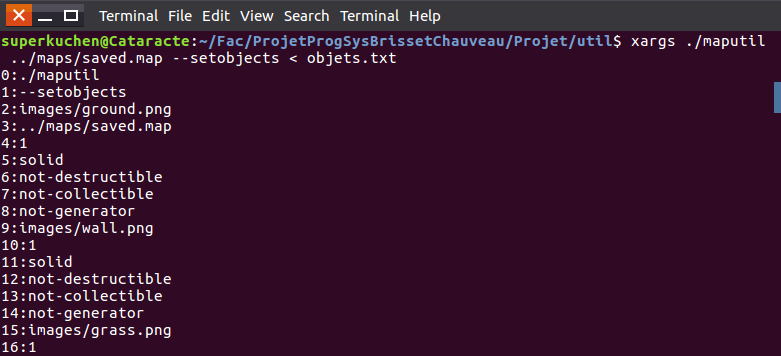
\includegraphics[scale=0.5]{erreurArgs.png}

\part{Gestion des temporisateurs}

\section{Choix d'implémentation}
Pour la temporisation, nous utilisons l'appel systéme \textbf{setitimer()} qui envoie un signal sigalrm pour un temps donné à la fonction par la structure itimer.
\newline La récuperation des signaux se fait via un thread ``démon'' qui, lorsqu'il recoit un signal sigalrm, appelle la fonction \textbf{sdl\_push\_event()} et ensuite émet un signal sigusr1.
\newline La gestion de plusieurs temporisateurs se fait grâce à l'implémentation d'une \textbf{file de priorité} qui nous permet de toujours avoir en tête de file la liste d'évenements qui se termine en premier. Cette liste contient un ou plusieurs événements qui se terminent en même temps ou dans un intervalle de temps proche du premier élément de cette liste .
\newline La fonction \textbf{defiler} est appelée lors de la réception du signal sigusr1, et permet de supprimer la première liste de la file. Dans le cas où il y a au moins deux éléments dans cette liste la fonction libère le premier évenement et émet un signal sigalrm pour que le démon puisse gérer cette événement . 

\section{Des difficultés}
La première difficulté était de trouver un moyen pour que le thread principal ne recupère pas le sigalrm, mais le thread démon. Cela à vite été résolu grâce à la fonction \textbf{pthread\_sigmask()} qui permet de bloquer différents signaux pour un thread.
\newline Ensuite, une autre difficulté était de bien faire la file de priorité. Ce probléme s'est résolu petit à petit en voyant les erreurs au fûr et à mesure que nous avancions .
\newline Le plus gros probléme a été la succession des temporisations, car nous n'arrivions pas à enchainer les temporisateurs avec la bonne valeur. Nous avons trouvé la solution grâce à l'aide d'un camarade qui nous a aidé à mieux comprendre la succession des temporisateurs, nous n'avions pas bien converti le temps de fin du temporisateur, que nous avions calculé.


\end{document}
